% !TEX root = document.tex

\chapter{\label{chap:treecomp}Compiling with Command Trees}

In this chapter we propose command trees as an improvement upon the \icode{Cps} data type of the previous chapter. The new compiler uses the \icode{Tree} and \icode{Tps} data type as IR. Compiler passes on the IR will have a type that looks like \icode{pass :: arg -> Tps cmd Val -> Tps cmd' Val}. Leaf nodes of the tree contain values of type \icode{Val}. \icode{arg} is used to model an effect. For example when closure converting \icode{arg} is a list of variable names in scope of type \icode{[String]}. These extra arguments are hidden by instantiating them with a starting value. For closure conversion the starting value would be an empty list. The differences between \icode{cmd} and \icode{cmd'} indicate what a pass does. Some care needs to be taken when splitting up commands into separate data types. We want to put constructors together which are transformed by the same compiler pass in order to maximize the information presented by the type of the pass.

\begin{figure}
\begin{gather*}
  String \xto{str2lam}\\
  Lam \xto{lam2tree}\\
  Tree \, Cmd \, Val \xto{tree2tps}\\
  T (Fix + Base) \xto{hClos}\\
  T (Record + Fix + Base) \xto{hRecord}\\
  T (Malloc + Fix + Base) \xto{swap}\\
  T (Fix + Malloc + Base) \xto{hFix}\\
  ([(String,[String],T (Malloc + Base))], T (Malloc + Base)) \xto{tps2wat}\\
  Wat \xto{show}\\
  String
\end{gather*}
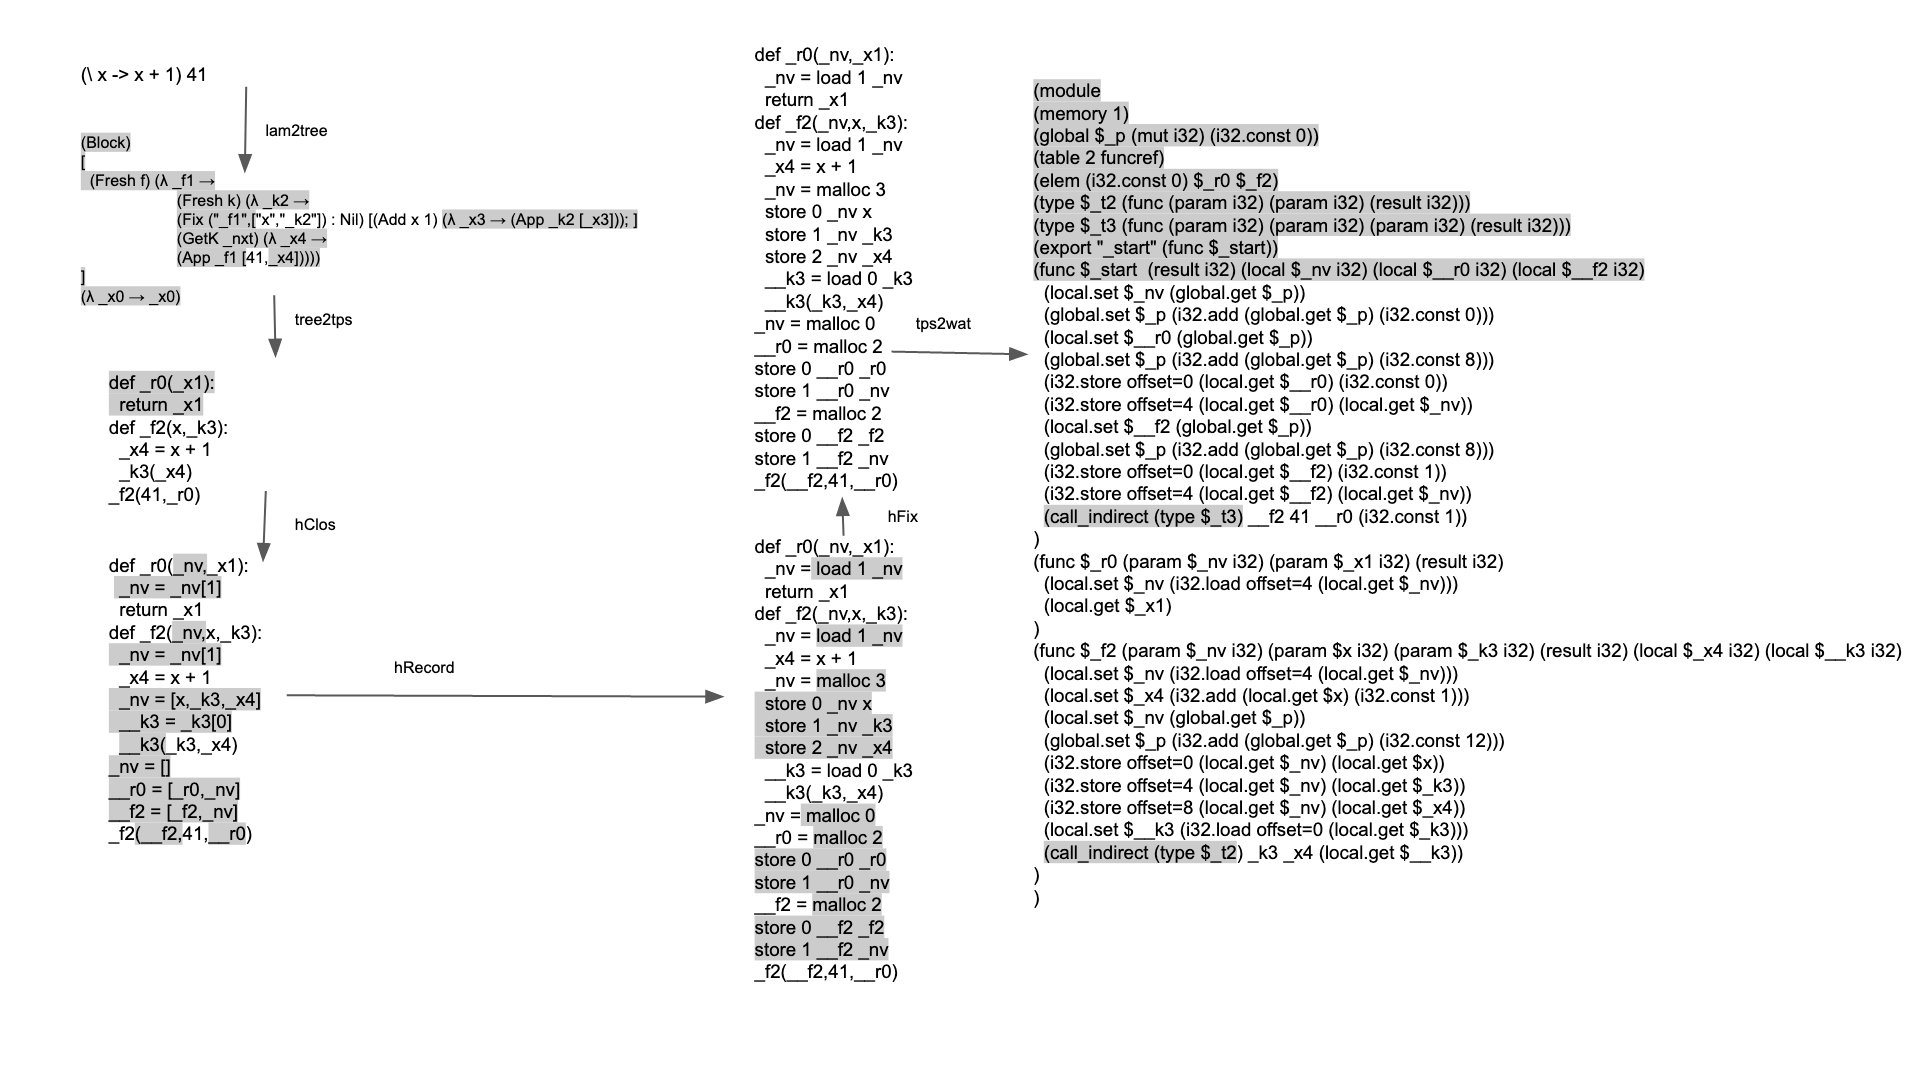
\includegraphics[width=1\textwidth]{./img/tps.png}
\caption{LamToWat Version 2: compiler organization. New pieces of code are highlighted in grey.}
\label{fig:lam2watv2org}
\end{figure}

We use the type synonym \icode{type T cmd = Tps cmd Val} to show the essence of the transformations. We notice that our compiler consist of more transformations than before. The increase in compiler steps does not mean an increase in complexity, but an increase in explicitness and declarativity. Some steps are almost trivial but the new type of \icode{Tps} gives the programmer information about the transformations. We combine different commands by using open unions ($+$ in the figure, and \icode{:+:} in code), these are discussed in subsection \ref{subsection:openunion}. \icode{Tree} is used in the front-end of the compiler, while \icode{Tps} is used in the back-end. Why we use these two data types is explained in the next section. You may already guess what the other commands are related to. We will see them in action in the next sections.

This chapter is structured in the same manner as the previous chapter: we will first discuss the new \icode{Tree} and \icode{Tps} data types and then examine their transformations.

\section{\label{section:commandtree}Command Trees}
Command trees are a data type used to sequence commands. A well known data type that is also capable of sequencing is a list. Command trees improve upon lists by adding subcontinuations, and by providing the ability to use the result of our command in the commands after that. Just like lists, command trees are monads. This allows us to bind command trees together easily and write functions using \icode{do}-notation.

Commands themselves are a syntactic representations of a monadic computations. In simpler terms this can be described as the meaning of a command is something that is left to the programmer. What a command does is implemented later in a function sometimes called a handler. Command trees are used to model effects in denotational semantics. We can write handlers for effects to create an interpreter. In this chapter we try to extend this approach to writing a compiler. We discuss the role of command trees in denotational semantics in more detail in section \ref{section:denotationalsemantics}.

The structure and monadic nature of command trees have already been discussed in \citetitle{commandtreespoulsen} \autocite{commandtreespoulsen}. A modified version of the discussion will be restated in this chapter for completeness. A command tree consists of two constructors: \icode{Leaf} and \icode{Node}. \icode{Leaf a} is the smallest form of command tree that exists and simply returns the value \icode{a}. A \icode{Node cmd ks k} command tree is somewhat more complex and is made up of three parts:

\begin{itemize}
\item A command \icode{cmd} that may have a signature,
\item A list of subcontinuations \icode{ks},
\item An optional continuation (also called join-point) \icode{k}.
\end{itemize}

We will call the data type \icode{Tree} a semantic command tree and \icode{Tps} a syntactic command tree. This means that continuations will have a arrow type \icode{a -> Tree cmd b} in \icode{Tree} and a tuple type where the left element is a \icode{String} indicating the variable name \icode{(String,Tps cmd b)} in \icode{Tps}. Syntactic command trees allow us to analyse variable bindings syntactically, something we need for (free) variable analysis. LamToWat needs this information to perform closure conversion.

Command trees are implemented using Haskell's GADTs. A GADT gives us the power to add more types to our IR. The notation of a GADT is somewhat different than the notation of a normal data type. After the \icode{data} keyword we specify a name and type parameters, a \icode{where} keyword follows. Then the different constructors of the GADT are declared. The constructors are given a name followed by \icode{::}. The types of the arguments follow, separated by \icode{->}. Finally, we declare the constructor with its type parameters, which can relate to the types of the arguments.

\subsection{\label{subsection:semantree}Semantic Command Tree}
A semantic command tree \icode{Tree} is defined by a GADT as follows.

\begin{lstlisting}[language=Haskell]
data Tree sig a where
  Leaf :: a -> Tree sig a
  Node :: sig n b p r q ->
          Vec n (p -> Tree sig r) ->
          Option b (q -> Tree sig a) ->
          Tree sig a
\end{lstlisting}

A semantic command tree does not know what set of commands is used. However, it does encode strong type constraints on its subcontinuations and continuation. To enforce these constraints we use a signature \icode{sig}. This way a command tells the semantic command tree what comes after itself. More formally a signature has type:

\begin{lstlisting}[language=Haskell]
type Sig = Nat -> Bool -> * -> * -> * -> *
\end{lstlisting}

A signature instance \icode{sig n b p r q} tells us the following things:

\begin{itemize}
\item The tag of the command and its enclosed parameters.
\item The number of subcontinuations \icode{n}.
\item If the command has a continuation.
\item The argument \icode{p} and return type \icode{r} of the subcontinuations.
\item The argument type \icode{q} of the continuation.
\end{itemize}

Without commands we can not do anything with our command trees. We will use a set of commands that reflect the constructors from the \icode{Cps} data type. We also define a number of extra commands that will help us compile. This progammifying or treeifying of a command or request is called lifting. This is called so because we 'lift' the expression into the monad.

\begin{lstlisting}[language=Haskell]
data Cmd :: Sig where
  -- cps commands
  Add   :: Val -> Val ->               Cmd Z     True  Void  Void Val
  App   :: Val -> [Val] ->             Cmd Z     False Void  Void Val
  Fix   :: Vec n (String, [String]) -> Cmd n     True  ()    Val  ()
  -- compilation commands
  GetK  :: String ->                   Cmd Z     True  Val   Val  Val
  SetK  :: String -> Val ->            Cmd Z     True  Val   Val  ()
  Block ::                             Cmd (S Z) True  ()    Val  Val
  Fresh :: String ->                   Cmd Z     True  Void  Void String
\end{lstlisting}

We can see that our original constructors \icode{Add}, \icode{App}, \icode{Fix} from the \icode{Cps} data type are here. Except the \icode{DONE} constructor will be modeled by \icode{Leaf}. The \icode{Val} type is the same as in \icode{Cps}. Our four extra commands represent a continuation store, command concatenation, and fresh variable name generation.

We take a look at the signatures of the commands to see how they are structured. The \icode{Block} and \icode{Fix} command are the only ones that have subcontinuations. The \icode{Void} type indicates that there is no subcontinuation. \icode{Fix} has a subcontinuation for every function definition. This is required by the constructor itself as the natural number \icode{n} appears in both the function name with arguments and subcontinuations. The \icode{App} command does not have a continuation, which will lead to some trouble when trying to concatenate it with other commands. The return type of commands indicates that commands will bind to a variable \icode{Val}, or only produce a side-effect \icode{()}.

We use helper functions to remove boilerplate and make the transformations more readable, e.g., \icode{add}, \icode{app}, etc. These are simple sugar that lift expressions into command trees. For example, the \icode{Add} command has sugared version \icode{add}.

\begin{lstlisting}[language=Haskell]
add :: Val -> Val -> Tree Cmd Val
add v1 v2 = Node (Plus v1 v2) Nil (Some Leaf)
\end{lstlisting}

Let's see how our example \icode{(\ x -> x + 1) 41)} translates to a semantic command tree. The translation is very similar to that of the \icode{Cps}. We use a \icode{Fix} command to create a function \icode{f} with argument \icode{x}. The body of this function adds \icode{x} and the number one \icode{1}. The continuation is a leaf node, which serves the same purpose as the \icode{DONE} constructor. The function name and arguments are separated by the function body, which is a vector of thunks (functions that take \icode{()} as argument). The continuation of our function node is an application node. Here we apply the function \icode{f} to the argument \icode{41}.
  
\begin{lstlisting}[language=Haskell]
Node (Fix (("f", ["x"]) ::: Nil)) ((\ () ->
  Node (Add (VAR "x") (INT 1)) Nil (Some (\ n -> Leaf n))) ::: Nil) (Some (\ () ->
Node (App (VAR "f") [INT 41]) Nil None))
\end{lstlisting}

Just like with \icode{Cps} we have a printed version of semantic command trees. The printed version looks like the written version we just examined.

\begin{lstlisting}[language=Haskell]
(Fix ("f",["x"]) : Nil) [(Add x 1) (λ _x0 → _x0); ] (App f [41])
\end{lstlisting}

\subsection{\label{subsection:syntree}Syntactic CPS Command Tree}
Syntactic command trees have, as their name implies, syntactic representation of name binding in their constructors. The signature types of continuations are dropped to make the tree specific to the notion of values in \icode{Cps}: \icode{Val}. The signature types that indicate the number of subcontinuations and the presence of a join-point remain. We require a function to translate from our semantic command trees to syntactic command trees. Moreover, a new set of commands need to be made for the syntactic trees. A syntactic command tree specialized for CPS \icode{Tps} is defined by a GADT as follows.

\begin{lstlisting}[language=Haskell]
data Tps sig a where
  Leaf :: a -> Tps sig a
  Node :: sig n b
       -> Vec n (Tps sig Val)
       -> Option b (String, Tps sig a)
       -> Tps sig a
\end{lstlisting}

The signature of \icode{Tps} has the following type.

\begin{lstlisting}[language=Haskell]
type Sig = Nat -> Bool -> *
\end{lstlisting}

A signature instance \icode{sig n b} tells us the following things:

\begin{itemize}
\item The tag of the command and its enclosed parameters.
\item The number of subcontinuations \icode{n}.
\item If the command has a continuation.
\end{itemize}

The set of syntactic commands does no longer require the commands related to compilation. These commands are given a syntactic representation within the tree. Therefore, our set of commands will match the original CPS commands almost completely with the exception of the \icode{DONE} expression. The commands are separated into modules. The separation is made with the compilation steps that follow in mind, which are mainly concerned with transforming functions. The \icode{VoidCmd} is used to write transformation generically. For example, we define a transformation of a command to another command as the function \icode{foo :: Tps (cmd :+: rest) Val -> Tps (cmd' :+: rest) Val}. This transformation should also work if the only command in the tree is \icode{cmd}. The tree would have type \icode{Tps cmd Val}, but this does not match because there is no \icode{rest}. This is where the \icode{VoidCmd} takes the place of \icode{rest}. This is some overhead of the way we defined our open unions.

\begin{lstlisting}[language=Haskell]
data Base :: Sig where
  App :: Val -> [Val] -> Base Z False
  Add :: Val -> Val ->   Base Z True 

data Record :: Sig where
  Record :: [Val] ->      Record Z True
  Select :: Int -> Val -> Record Z True

data Fix :: Sig where
  Fix :: Vec n (String,[String]) -> Fix n True

data Malloc :: Sig where
  Malloc :: Int ->               Malloc Z True
  Load   :: Int -> Val ->        Malloc Z True
  Store  :: Int -> Val -> Val -> Malloc Z True

data VoidCmd :: Sig where
\end{lstlisting}

If we look at the example \icode{(\ x -> x + 1) 41}, we will see that it is very similar to the semantic counterpart. The main difference is that semantic variables have been replaced with strings.

\begin{lstlisting}[language=Haskell]
Node (L (Fix (("f", ["x"]) ::: Nil)))
((Node (R (Add (VAR "x") (INT 1))) Nil (Some ("n", Leaf (VAR "n")))) ::: Nil) (Some ("",
Node (R (App (VAR "f") [INT 41])) Nil None))
\end{lstlisting}

The printed version of syntactic command trees is exactly the same as that for \icode{Cps}, because the compilation commands have been dropped.

\begin{lstlisting}[language=Haskell]
def f(x):
  n = x + 1
  return n
f(41)
\end{lstlisting}

\subsubsection{\label{subsection:openunion}Open Unions or Extensible Sums}
In order to compile \icode{Lam} into \icode{Wat} we will have to make use of all our \icode{Tps} command modules. We will combine our commands using an open union or extensible sum data type. An open union can be viewed as a list of data types. More precisely, it is a binary tree which has data types as leaf nodes. \icode{:+:} is right-associative and has two constructors \icode{L} and \icode{R}, which inject a data type into the left or right side of the tree, respectively. Note that we can nest instances of open unions to create open unions. Open unions make our command tree somewhat modular, because we can add new commands to an existing union to represent new language features.

\begin{lstlisting}[language=Haskell]
data (:+:) :: Sig -> Sig -> Sig where
  L :: sigl n b -> (sigl :+: sigr) n b
  R :: sigr n b -> (sigl :+: sigr) n b
\end{lstlisting}

\begin{lstlisting}[language=Haskell]
class (sub :: Sig) :<: (sup :: Sig) where
  inj :: sub n b -> sup n b
\end{lstlisting}

We use smart constructors to mitegate the syntactic overhead of injecting \autocite{DBLP:conf/haskell/WuSH14, DBLP:conf/popl/LiangHJ95} even further. For example to lift our \icode{Add} command into the command tree we can define the following function. The constraint \icode{Base :<: cmd} ensures that \icode{Add} is located somewhere in the commands of the command tree.

\begin{lstlisting}[language=Haskell]
add_ :: Base :<: cmd => Val -> Val -> String -> Tps cmd ()
add_ v1 v2 x = liftT (inj (Add v1 v2)) Nil x (Leaf ())
\end{lstlisting}

We will rarely use the original commands and mostly use their smart constructors when writing our tree transformations. The \icode{(\ x -> x + 1) 41} example will be represented as follows. Notice that it is written with \icode{do} notation, because we are working inside a monad. The type of the command of this tree is not concretely instantiated. Instead two constraints are added and we get a tree of type \icode{(Fix :<: cmd, Base :<: cmd) => Tps cmd Val}, indicating that both \icode{Fix} and \icode{Base} commands are injected somewhere in \icode{cmd}.

\begin{lstlisting}[language=Haskell]
fix_ (("f",["x"]) ::: Nil)
  ((add (VAR "x") (INT 1) "n" (done (VAR "n"))) ::: Nil)
app (VAR "f") [INT 41]
\end{lstlisting}

Extensible sums should behave like sets, but are implemented as binary trees. This means that the order of commands matters, e.g., \icode{A :+: B} is not the same as \icode{B :+: A} in the eyes of the Haskell type system. To mitigate this we can write helper functions that transform the structure of our extensible sums. In LamToWat we use the \icode{swap} function which is defined as follows. 

\begin{lstlisting}[language=Haskell]
fix_ (("f",["x"],do
      add_ (VAR "x") (INT 1) "n"
      done (VAR "n"))
      ::: Nil)
app (VAR "f") [INT 41]
\end{lstlisting}

\section{\label{section:treensforms}Tree Transformations}
Transformations for the new version of LamToWat will be implemented as Haskell functions. Since command trees are monads, we will program mostly in the monad using \icode{do}-notation. 

\subsection{\label{subsection:cpsconvert2}CPS Conversion}
Using \icode{Tree}, we can define an improved CPS conversion. The function is easier to read and write. We no longer have a metacontinuation hidden inside a continuation monad. This simplifies the notation significantly. We still operate in a monad, however, this monad is the command tree. The order of our listed operations matches the order of our final program more closely. There are some details that spoil the declarativity of our conversion somewhat. The advantages and disadvantages of our new approach become clear when we examine the conversion of a lambda abstraction in comparison to the one in the previous version of LamToWat.

\begin{lstlisting}[language=Haskell]
lam2tree :: Lam -> Tree Cmd Val
lam2tree (Var x) = return (VAR x)
lam2tree (Num i) = return (INT i)
lam2tree (Lam x e) = do
  f <- fresh "f"
  k <- fresh "k"
  fix ((f,[x,k],do
           v <- lam2tree e
           app (VAR k) [v])
       ::: Nil)
  return (LABEL f)
lam2tree (App e1 e2) = block (do
  v1 <- lam2tree e1
  v2 <- lam2tree e2
  k <- getk "_nxt"
  app v1 [v2,k])
lam2tree (Add e1 e2) = do
  v1 <- lam2tree e1
  v2 <- lam2tree e2
  add v1 v2
\end{lstlisting}

We take a look at the conversion of \icode{Lam}. We generate a fresh function variable \icode{f} and continuation variable \icode{k}. We use these variables to create a function with name \icode{f} that has as argument the original variable and a continuation named \icode{k}. The body of the function will be the converted original body and a final statement that applies the continuation to the resulting variable. Finally, we return a \icode{LABEL} with the function name.

We convert our example lambda expression \icode{(\ x -> x + 1) 41} to obtain the following result. The most notable novelty is the use of a \icode{Block}. Blocks are used to bind parts of code together and replace the metacontinuation of the original version. If we take the code outside the block it would end with an application of \icode{_f1}. Since applications do not have a continuation, any code after it would be discarded. In our case the application is the last thing that happens, so it does not really matter, but when we nest more than one application in our expression it becomes a problem. Continuations will be dropped. This is not the behavior we want, so we use \icode{block}s instead. We also see that there are still \icode{fresh} commands in the tree. These will be handled when transforming to \icode{Tps} in the next transformation.

When we transform function application we need access to the next continuation and pass it to the transformed function \icode{_f1}. We obtain the next continuation with \icode{GetK _nxt}. The variable \icode{_nxt} is set to the continuation of a block when entering that block. The old 'next' continuation is saved and restored when exiting the block. In this case the continuation is \icode{_x0}, which just returns the value given to it. We can see the resemblance with continuation functions and blocks. This is not incidental: blocks will be compiled into continuation functions. So why do we not just use continuation functions? Because we do not have access to continuations yet. We are still operating on \icode{Lam}, without the help of a continuation monad. After we have transformed into a command tree we will be able to access the continuation of a command.

\begin{lstlisting}[language=Python]
(Block) 
[
  (Fresh f) (λ _f1 →
    (Fresh k) (λ _k2 →
      (Fix ("_f1",["x","_k2"]) : Nil) [(Add x 1) (λ _x3 → (App _k2 [_x3])); ] 
        (GetK _nxt) (λ _x4 → 
          (App _f1 [41,_x4]))))
] (λ _x0 → _x0)
\end{lstlisting}

\subsection{\label{subsection:semtosyn}Tree Compilation}
The \icode{Tree} that is output by \icode{lam2tree} contains commands that represent effects. We will need to handle these commands and instantiate name binding commands with generated variables before we can closure convert. By handling the syntactic representation of effects we give meaning to them. The transformation is called \icode{lam2tree} and is performed using monad \icode{M}. The monad \icode{M} provides a number that is used as a postfix for generating fresh variable names and an environment that associates \icode{String}s with \icode{Val}s.

\begin{lstlisting}[language=Haskell]
type M = StateT Int (Reader [(String,Val)])
\end{lstlisting}

\begin{lstlisting}[language=Haskell]
t2t :: Tree Cmd Val -> M (Tps (Fix :+: Base :+: VoidCmd) Val)
t2t (Leaf x) = return (done x)
t2t (Node (T.Add v1 v2) Nil (Some k)) = do
  x <- fresh "x"
  k' <- t2t (k (VAR x))
  return (add v1 v2 x k')
t2t (Node (T.App v vs) Nil None) =
  return (app v vs)
t2t (Node (T.Fix fxs) bs (Some k)) = do
  bs' <- mapM (\ b -> t2t (b ())) bs
  k' <- t2t (k ())
  return (fix' fxs bs' k')
t2t (Node (T.SetK x v) Nil (Some k)) =
  local ((x,v):) (t2t (k ()))
t2t (Node (T.GetK x) Nil (Some k)) = do
  nv <- ask
  case lookup x nv of
    Just v -> t2t (k v)
    Nothing -> error (x ++ " is not in env " ++ show nv)
t2t (Node T.Block (b ::: Nil) (Some k)) = do
  r <- fresh "r"
  x <- fresh "x"
  b' <- local (("_nxt",LABEL r):) (t2t (do v <- b (); T.app (LABEL r) [v]))
  k' <- t2t (k (VAR x))
  return (fix' ((r,[x]) ::: Nil) (k' ::: Nil) b')
t2t (Node (T.Fresh x) Nil (Some k)) = do
  f <- fresh x
  t2t (k f)
\end{lstlisting}

The compilation of the \icode{Fresh} command seems trivial, because we use the helper function \icode{fresh}. This helper function should not be confused by the sugared version of the \icode{Fresh} command. This function updates the state integer of \icode{M} and returns a fresh variable (in this case a string).

The compilation of \icode{Add} shows the instantiation of variables in the metalanguage with variables in the syntactic command trees. We generate a fresh variable \icode{x}, pass it to the continuation and compile the continuation, and finally plug the result into the syntactic command tree.

The \icode{Setk} and \icode{Getk} commands update and fetch named continuations. In our case there is only a continuation that is named \icode{_nxt}. The \icode{Block} command tells us to compile the continuation \icode{k} by passing it \icode{VAR x} and wrap it in a continuation function with name \icode{r} and argument {x}. We set the continuation \icode{_nxt} to the function label \icode{LABEL r}. We extend the body of the block with a final application of the continuation function \icode{r} to the result \icode{v} and compile with the updated continuation list. Finally, we create the continuation function and give it the compiled body \icode{b'} as continuation.

After tree compilation we obtain a \icode{Tps} with the commands \icode{Fix} and \icode{Base}. Our example \icode{(\ x -> x + 1) 41} now looks the same as \icode{Cps} after CPS conversion. We have done two tranformations to obtain the same result. However, these transformations are significantly easier to write and the conversion from \icode{Tree} to \icode{Tps} only has to be written once if we keep the command set that \icode{Tree} has now. We show the printed version of \icode{Tps} (and \icode{Cps}) for reference here.

\begin{lstlisting}[language=Haskell]
def _r0(_x1):
  return _x1
def _f2(x,_k3):
  _x4 = x + 1
  _k3(_x4)
_f2(41,_r0)
\end{lstlisting}

\subsection{\label{subsection:closconvert2}Closure Conversion}
Now that we have eliminated our effectful commands we can closure convert our tree. We will follow the same approach as in the previous version: collect names of expression and use these to construct records. We will make the assumption that the only place where expressions are named (and thus our environment is extended) is in the join-point of a node and in functions. We do not hoist our function definitions to the top level immediately. We need an extra function for this. Separating these two transformations also gives as a chance to better describe the type of the command tree before and after.

Using monadic helper functions we can make this transformation somewhat easier to read. We see that the transformation only really effects \icode{Fix} and \icode{App} nodes. The type of \icode{hClos'} shows that we transform \icode{Fix} and \icode{Base} commands by adding a \icode{Record} command to our command tree. In the organization of our compiler we see the function \icode{hClos} used instead of \icode{hClos'}. \icode{hClos} is simply \icode{hClos'} instantiated with an empty list, e.g., \icode{hClos = hClos' []}.

\begin{lstlisting}[language=Haskell]
hClos' :: [String] -> Tps            (Fix :+: Base :+: cmd) Val -> 
                      Tps (Record :+: Fix :+: Base :+: cmd) Val
hClos' nv (Node (L (Fix fxs)) bs (Some (_,k))) = do
  let fxs' = mapV (\ (f,as) -> (f,"_nv":as)) fxs
      bs' = zipWithV (\ (f,as) b -> do
                       select_ 1 (VAR "_nv") "_nv"
                       zipWithM_ (\ i x ->
                                    if x `elem` as
                                    then return ()
                                    else select_ i (VAR "_nv") x) [0..] nv
                       hClos' (nv ++ as) b) fxs bs
  fix' fxs' bs' (hClos' nv k)

hClos' nv (Node (R (L (App v vs))) Nil None) = do
  record_ (map VAR nv) "_nv"
  vs' <- mapM (\ v -> case v of
                  LABEL f -> do
                    let _f = "_" ++ f
                    record_ [v,VAR "_nv"] _f
                    return (VAR _f)
                  _       -> return v) vs
  case v of
    LABEL f -> do
      let fc = "_" ++ f
      record_ [v,VAR "_nv"] fc
      app v (VAR fc:vs')
    VAR f -> do
      let fp = "_" ++ f
      select_ 0 v fp
      app (VAR fp) (v:vs')
hClos' nv (Leaf v) = Leaf v
hClos' nv (Node cmd ks k) =
  Node (R cmd) (fmap (hClos' nv) ks)
    (fmap (\ (x,k) -> (x, hClos' (nv ++ if null x then [] else [x]) k)) k)
\end{lstlisting}

We see how our nested example \icode{(\ x y -> x + y) 13 29} looks after closure conversion. Functions have an extra \icode{_nv} argument. Bodies of functions are prefixed with opening the closure and postfixed with creating closures before calling another function. In the previous version of LamToWat we did not get to see this rendering of our example, because it was hoisted immediately.

\begin{lstlisting}[language=Python]
def _r0(_nv,_x1):
  _nv = _nv[1]
  return _x1
def _r2(_nv,_x3):
  _nv = _nv[1]
  _nv = [_x3]
  __r0 = [_r0,_nv]
  __x3 = _x3[0]
  __x3(_x3,29,__r0)
def _f4(_nv,x,_k5):
  _nv = _nv[1]
  def _f6(_nv,y,_k7):
    _nv = _nv[1]
    x = _nv[0]
    _k5 = _nv[1]
    _x8 = x + y
    _nv = [x,_k5,y,_k7,_x8]
    __k7 = _k7[0]
    __k7(_k7,_x8)
  _nv = [x,_k5]
  __f6 = [_f6,_nv]
  __k5 = _k5[0]
  __k5(_k5,__f6)
_nv = []
__r2 = [_r2,_nv]
__f4 = [_f4,_nv]
_f4(__f4,13,__r2)
\end{lstlisting}

Before we hoist our function definitions to the top level we can transform our \icode{Record} commands into \icode{Malloc} commands. Here we see that we can fix our shortcoming of repeated constructors quite easily with command trees. We can focus on a particular command and translate it into its lower-level counterpart. In this case only \icode{Record} as truly translated as \icode{Select} and \icode{Load} have a one-to-one mapping.

\begin{lstlisting}[language=Haskell]
hRecord :: Tps (Record :+: cmd) Val -> Tps (Malloc :+: cmd) Val
hRecord (Node (L (Record vs)) Nil (Some (x,k))) = do
  malloc_ (length vs) x
  zipWithM_ (\ i v -> store_ i (VAR x) v) [0..] vs
  hRecord k
hRecord (Node (L (Select i v)) Nil (Some (x,k))) =
  load i v x (hRecord k)
hRecord (Leaf v) = Leaf v
hRecord (Node (R cmd) ks k) = Node (R cmd) (fmap hRecord ks) (fmap (fmap hRecord) k)
\end{lstlisting}

Hoisting is done with the \icode{hFix} function. We will need to be able to open the join-point of a \icode{Node} of our command tree in order to be able to hoist, because it is a non-local transformation. A non-local transformation affects the entire tree. In the case of hoisting we are chopping up the tree into individual commands, separating the \icode{Fix} commands and putting them into a list, and glueing the other commands back together to form a new tree.

The resulting type is a tuple of a command tree function list and a command tree representing something like the actual program. The type clearly indicates that functions no longer contain other functions. We only have \icode{Tps} without \icode{Fix} commands in combination with a function name (\icode{String}) and function arguments (\icode{[String]}) to represent a function.

\begin{lstlisting}[language=Haskell]
hFix :: Tps (Fix :+: cmd) Val -> ([(String,[String],Tps cmd Val)],Tps cmd Val)
hFix (Leaf v) = ([],Leaf v)
hFix (Node (R cmd) ks k) = case fmap (fmap hFix) k of
  Some (x,(fs,k')) -> (fs++fs',Node cmd ks' (Some (x,k')))
  None             -> (    fs',Node cmd ks' None)
  where ks' = fmap (snd . hFix) ks
        fs' = concat (toList (fmap (fst . hFix) ks))
hFix (Node (L (Fix fxs)) bs (Some ("", k))) = let (fs,k') = hFix k in (fs'++fs,k')
  where fs' = concatMap 
               (\ ((f,as),b) -> let (fs,b') = hFix b in (f,as,b') : fs) 
                (zip (toList fxs) (toList bs))
\end{lstlisting}

The result of \icode{hFix} of the example \icode{(\ x -> x + 1) 41} looks as follows. It is the same as \icode{Cps} after the closure conversion step except for the replacement of records and selects with mallocs, loads, and store.

\begin{lstlisting}[language=Haskell]
def _r0(_nv,_x1):
  _nv = load 1 _nv
  return _x1
def _f2(_nv,x,_k3):
  _nv = load 1 _nv
  _x4 = x + 1
  _nv = malloc 3
  store 0 _nv x
  store 1 _nv _k3
  store 2 _nv _x4
  __k3 = load 0 _k3
  __k3(_k3,_x4)
_nv = malloc 0
__r0 = malloc 2
store 0 __r0 _r0
store 1 __r0 _nv
__f2 = malloc 2
store 0 __f2 _f2
store 1 __f2 _nv
_f2(__f2,41,__r0)
\end{lstlisting}

\subsection{\label{subsection:emit2}Emitting}
The emit step now becomes even more trivial, as we have also eliminated records from our command tree and replaced them with malloc commands. We include this step for completeness and testing purposes. We could use the command tree output by \icode{hFix} to generate WebAssembly code. The mapping is one-to-one for expressions: every remaining tree command has a \icode{Wat} counterpart. However, the transformation of \icode{Val}s does need to change labels into integers.

\begin{lstlisting}[language=Haskell]
type Tps' = Tps (Malloc :+: Base :+: VoidCmd) Val

tps2wat :: ([(String,[String],Tps')],Tps') -> Wat
tps2wat (fs,e) = Module fs' (go e)
  where ns :: [String]
        ns = map (\ (f,as,b) -> f) fs

        fs' :: [(String,[String],Exp)]
        fs' = map (\ (f,as,b) -> (f,as,go b)) fs

        go :: Tps' -> Exp
        go (Leaf v)                                    = W.Done (vo v)
        go (Node (L (Malloc i))      Nil (Some (x,k))) = W.Malloc i x (go k)
        go (Node (L (Load i v))      Nil (Some (x,k))) = W.Load i (vo v) x (go k)
        go (Node (L (Store i s t))   Nil (Some (_,k))) = W.Store i (vo s) (vo t) (go k)
        go (Node (R (L (Add v1 v2))) Nil (Some (x,k))) = W.Add (vo v1) (vo v2) x (go k)
        go (Node (R (L (App v vs)))  Nil None)         = W.App (vo v) (map vo vs)
        
        vo v = case v of
          LABEL x -> INT (fromJust (x `elemIndex` ns))
          _       -> v
\end{lstlisting}

\section{\label{section:commandtrees}Command Tree Improvements}
In this section we will explore the design space for command trees and discusss the shortcomings of the second version of LamToWat. During the development of the LamToWat compiler a number of different command trees were examined to see if they could provide us with a replacement for \icode{Cps}. We will discuss some of the relevant ones here.

% blocks
Although command trees provide a useful abstraction for language implementers, it does require knowledge of the block model for control flow. In the original version of LamToWat CPS conversion is implemented using a metacontinuation. This metacontinuation indicates what a program does next. When we transform a application we have to construct a return point function and pass it as the last argument to the new application. These manipulations of control flow become even more non-trivial when implementing imperative language constructs such as \icode{while} and \icode{for}. Moreover, when we have to use multiple metacontinuations in case we want to throw exceptions or break from a \icode{while} loop, the bookkeeping of metacontinuations becomes cumbersome. Command trees help the programmer somewhat by having these metacontinuations live inside the tree. The language implementer will still need to wrap certain parts of code inside a block and fetch the right continuation at the right point. The real burden is now put on the compiler writer, who has to compile the semantic command tree to a syntactic one.

% interpreter + morphism
In order to check intermediate results of the compiler we would like to have an interpreter for \icode{Tree} and \icode{Tps}. We now only have a pretty printer for both data types, but we want to be able to map \icode{Tree} and \icode{Tps} to a certain domain. The modular nature of \icode{Tps} requires some attention to make the interpreter modular as well. We would also like a function that transforms \icode{Tps} back into \icode{Tree} for the right set of commands. This would show the morphism between the two and give another check of the compilation process.

% type constraints
Our command trees have some types, but we would like our types to do even more. For example we want a type to indicate that an expression is closed after closure conversion, i.e., it does not have any free variables. Transforming syntactic command trees into semantic ones would function as a sort of type checking function. Typing closure conversion has been studied in Haskell and other languages \autocite{DBLP:conf/haskell/GuillemetteM07, DBLP:conf/pldi/Chlipala07, DBLP:conf/popl/MorrisettWCG98}. We tried to implement something similar in LamToWat but found Haskell's type system uncooperative.

% better open unions
The implementation of open unions we have used for making \icode{Tps} modular can be improved. There is still some extra work required of the programmer, e.g., using the function \icode{swap} before being able to apply \icode{hFix}. Open unions should behave like real sets and not suffer from their implementation as lists. There are some other implementations of open unions in the Haskell language which may provide the functionality we require \autocite{extensible-effects, open-union}.

\section{\label{section:summarytree}Chapter Summary}
In this chapter we have shown how the three shortcomings of our original compiler are eliminated by using command trees as IR. Each of the shortcomings addressed at the end of the previous chapter \ref{section:summarycps} is alleviated as follows. 

\begin{itemize}
\item CPS conversion becomes easier to specify by using blocks in \icode{lam2tree}
\item The type of the output of \icode{hFix} indicates that functions are no longer nested
\item \icode{hRecord} only transforms records and thus removes duplicate constructors
\end{itemize}

We separated \icode{Cps} into two command trees: semantic and syntactic. Semantic command trees give us the power to write a declarative CPS conversion function, improving the front-end of LamToWat. Syntactic command trees specific to \icode{Cps} allow the programmer to write modular, declarative transformations in the back-end of LamToWat without losing the ability to do variable analysis.

We can combine commands to create a modular approach to compilation. With the help of smart constructors and destructors we reduce syntactic overhead. More transformations are performed on the command tree than on \icode{Cps}, because we have to handle effects ourselves. Although it requires a little more effort on behalf of the programmer, it also provides a method to make transformations explicit and declarative. In the next chapter we will discuss the background of command trees and their context: modular denotational semantics.
